
\newpage
\chapter{Background}

\section{High Performance Computing}

Accelerated Computing also known as computational acceleration has led to an era of high performance computing (a.k.a HPC). Moore's law has been widely accepted as an industry standard and these industries were highly dependent on Moore's law for better performance and improved efficiency. It was cited by most of the semiconductor manufacturers as they strive to increase computational power. Every year, the transistors that were being added on the silicon area were very fast and consumed less amount of power. But, in recent years, Moore's Law has slowed down by a considerable amount since as the number of the transistor on the chip increases, the frequency stopped scaling. Hence, it became very difficult to extract the performance from a single core processor (sequential CPU). Moreover, single processor ran into memory wall and power wall issues. Thus, adding more CPU cores was a solution from where the multicore processor emerged. However, with multiple CPU cores, it became difficult to gain better performance out of these chips. The challenge was writing the code that can run across multiple cores simultaneously. Moreover, some instructions can't run simultaneously at all. So, the computing world ended up with multicore CPUs that could not accelerate all types of code. This made the designer’s job even harder. Simply adding cores resulted into waste of transistors and raised the cost to manufacture the processor without much benefit. Failure to improve the performance of CPU, without affecting power budgets or using extremely complicated design methods resulted in the industry hitting a brick wall.

“Accelerated Computing has reached a tipping point in the High-Performance Computing. Within a year or two, the majority of the system will be equipped with accelerators”. \cite{3}

Heterogenous computing refers to systems that make use of more than one kind of processors. Performance gain or energy efficiency is achieved in these systems by adding dissimilar coprocessors for handling multiple type of tasks using their specialized computational/processing capabilities. Accelerated computing is a computing model used for accelerating applications in engineering and scientific domains wherein the computations are performed on specialized processors accelerators. It makes use of heterogeneous computing systems for improving the performance of application in which a lot of data is executed in parallel. The basic idea is to execute the code that is suitable for a processor. For example, sequential code with a lot of control instructions and branches would be preferred to run over a CPU since they would provide better performance for this kind of code, whereas computation which is highly parallel with very less branching conditions would be well suited for execution on the accelerator.


\section{FPGA Virtualization for High Performance Computing}

Virtualization of FPGA using the FPGA overlays delivers high performance for application acceleration \cite{4}. With the increasing complexity of FPGA platforms, it is being said that the use of overlay architecture will become mainstream. Overlay architecture can enable widespread use of the FPGAs in accelerated computing. FPGAs make the full utilization and advantage of Moore's Law improvements in semiconductor technology \cite{5}. Reconfigurable platforms consisting of general-purpose processors along with the programmable logic have been introduced by the major FPGA vendors like Xilinx and Altera. FPGAs are used for high speed computations for the data parallel applications. However, it remains difficult to develop an accelerator using Hardware Description Language (HDL). It requires expertise in hardware designing performing implementation and debugging for building hardware. Hardware design, design productivity and long compilation times are few of the barriers that restricts the use of FPGA in general purpose computing.

FPGA virtualization using Overlay architecture offers the advantage of the fast compilation, run-time management and software-like programmability because of their improved design productivity and high-level design abstraction \cite{6}, \cite{7},\cite{8}. Other benefits include better design reuse, application portability across platforms and rapid reconfiguration that is much faster than partial reconfiguration on fine grained FPGAs. Integrating overlays with memory subsystem and processor is important to enable sharing and management of limited overlay resources. Overlays exhibit features independent from the host FPGA. Soft processors can extend the capability of embedded hard vector processors in FPGA like Xilinx Zynq.

In this thesis work, we are going to use an overlay architecture known as MXP soft-processor used for high performance computing in our experiments while analysing the runtime, speedup and throughput obtained. It is a soft vector processor developed by Vectorblox Computing Inc \cite{9} and is classified as Single Instruction, Multiple Data (SIMD) Stream processor. It is provided as an IP core which can be instantiated over the FPGA. It provides the acceleration of the data parallel operations. MXP Vectorblox can be programmed in C/C++ and provides different C/C++ APIs support. This helps to program it easily rather than struggling a lot with Hardware Description Languages like VHDL or Verilog. For using an accelerator over FPGA, the hardware designing flow requires to go through a long design cycle (taking up hours to weeks) whereas on the other hand using MXP, all we need to do is to alter the given software code. MXPs parameterized design helps user to specify the amount of parallelism needed, which can range from 1 to 128. It includes a parallel access local scratchpad memory which holds the data and a high-throughput Direct Memory Access (DMA). MXP can be easily instantiated in the existing Xilinx and Altera development boards, simplifying the development.

In our work we have used Xilinx Zynq 7020 SoC \cite{10} heterogeneous computing platform wherein the MXP soft-processor is instantiated on its programmable logic fabric. Now, we will discuss about the hardware platform which we have used in detail.


\section{Zynq-7000 SOC Board}

Xilinx ZedBoard is a SOC development board which is based on Xilinx Zynq-7000 All Programmable SoC (AP SoC) \cite{11}. ZedBoard is a platform which is partitioned into Processing system (PS) consisting of one or multiple processors along with memory interfaces, bus and peripherals and the Programmable Logic. It provides a way in which even a customized hardware can be instantiated. These two parts are connected via high throughput interconnect to maximize communication bandwidth. ZedBoard features are shown below in table~\ref{zz:123}.

\begin{table}[htbp]
	\centering
	\begin{adjustbox}{width=.6\textwidth}
		\small
	
	\begin{tabular}{rl}
		\toprule
		\multicolumn{1}{l}{\textbf{Feature }} & \textbf{Description} \\
		\midrule
	    \multicolumn{1}{l}{Processor } & Zynq-7000 AP SoC XC7Z020-CLG-484-1 \\
		\midrule
	    \multicolumn{1}{l}{Memory } & 512 MB DDR3 \\
	      & 256 MB Quad-SPI Flash \\
	      & 4.0 GB SD card \\
		\midrule
	    \multicolumn{1}{l}{Communication} & Onboard USB-JTAG Programming \\
	      & USB OTG 2.0 and USB-UART \\
	      & 10/100/1000 Ethernet \\
		\midrule
	    \multicolumn{1}{l}{Expansion Connectors} & Expansion connectors  \\
	      & FMC-LPC connector  \\
	      & Five Pmod compatible header(2x6) \\
	      & Agile Mixed Signalling (AMS) header \\
		\midrule
	    \multicolumn{1}{l}{Clocking } & 33.33 MHz clock source for PS \\
	      & 100 Mhz oscillator for PL  \\
		\midrule
	    \multicolumn{1}{l}{Display } & HDMI output supporting 1080p60 with 16-bit \\
	      & YCbCr \\
	      & 4:2:2 mode color  \\
	      & VGA output (12-bit resolution color) \\
		\midrule
	    \multicolumn{1}{l}{Configuration and Debug} & Onboard USB-JTAG interface \\
	      & Xilinx Platform Cable JTAG connector \\
		\midrule
	    \multicolumn{1}{l}{General Purpose I/O} & Eight user LEDs  \\
	      & Seven push buttons \\
	      & Eight DIP switches \\
		\bottomrule	
	\end{tabular}%
    \end{adjustbox}
  \caption{ZedBoard Features}
  \label{zz:123}%
   \end{table}%



Figure~\ref{zed:blk} represents ZedBoard block diagram \cite{12}. It gives a brief idea about the Zynq xc7z020-clg484 System On Chip Development Board.

\begin{figure}
	\centering
	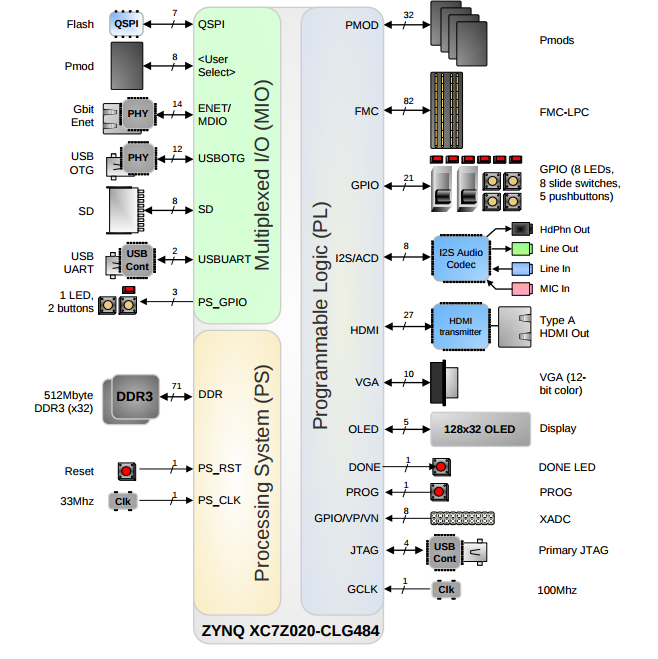
\includegraphics[width=0.9\textwidth]{images/zedboard_block.png}
	\caption{ZedBoard Block Diagram\cite{12}}
	\label{zed:blk}
\end{figure}

FPGA fabric provides the power of reconfigurability along with application specific acceleration while letting the processor execute control intensive tasks. Xilinx Zynq ZedBoard is a development and evaluation board which is based on Zynq-7000 All Programmable SoC architecture. It consists of Zynq Z7020-clg484 of speed grade -1(667 MHz) containing dual core ARM-Cortex A9 based processing system(PS) and PL fabric in one package \cite{13}. The PS consists of a floating-point unit (double precision), DMA controller, 512 MB DDR RAM, commonly used peripherals and external memory interfaces. The components of PS are listed as below:


\begin{itemize}
	\item Two ARM Cortex-A9 cores that are run-time configurable as a single processor.
	\item NEON 128b SIMD coprocessor and VFPv3 per processor.
	\item 512KB L2 cache that is shared between the processors.
	\item 32KB instruction and L1 data caches per processor.
	\item Snoop Control Unit (SCU) and the ACP for cache coherent accesses.
	\item On-Chip Memory (OCM) with capacity of 256KB.
	\item DMA controller with four channels for PS and PL.
	\item DDR controller.
	\end{itemize}

The PL is made up of Artix 7 FPGA fabric \cite{13}. It has 6-input lookup tables (LUTs) and 36kb Block RAMs which can be configured as two 18 Kb blocks. The processor in the system is first booted and PL is configured as a part of boot process or can be configured sometime later in the future. PL can be either reconfigured completely or partially by making use of the partial reconfiguration (PR) feature. The PL configuration data is referred to as bitstream. PL is useful for real-time applications as it has predictable latency. Power can be managed by powering down the PL as it has a different power domain than the PS. The PL has a rich architecture capable of user configuration which are listed below:

\begin{itemize}
\item Configurable logic blocks (CLB) with 6-input lookup table (LUT).
\item DSP48E1 Slices consisting ALU useful for Digital signal processing.
\item 36KB block RAM with capability of dual port.
\item Low jitter clock distribution and low skew.
\item High performance I/Os that can be configured.
\end{itemize}

The ARM based reconfigurable system on ZedBoard makes use of multiple AXI interfaces for communication between the PS and the PL. Each interface provides AXI channels, which helps in efficient data transfer and eliminates performance bottlenecks for memory and I/O. There are three types of AXI interfaces to the fabric mentioned below:

\begin{itemize}
\item AXI GP - Two 32-bit AXI master and two 32-bit AXI slave General purpose (GP ports).
\item AXI HP - Four 32-bit/64-bit configurable, AXI slave High Performance (HP) ports which are buffered along with direct access to DDR and OCM.
\item AXI ACP - One 64-bit AXI Accelerator Coherency Port (ACP) slave interface ensuring access to memory is coherent. AXI ACP - One 64-bit AXI Accelerator Coherency Port (ACP) slave interface.
\end{itemize}

\begin{figure}
	\centering
	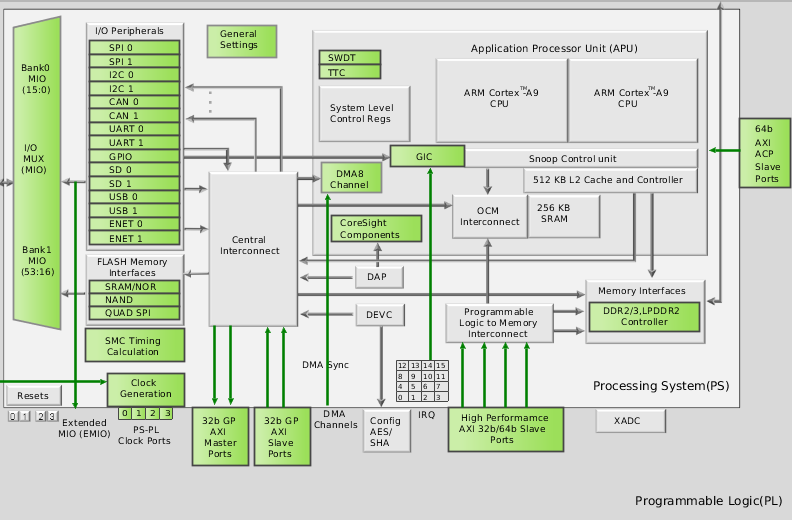
\includegraphics[width=0.9\textwidth]{images/zynqblockdiagram.png}
	\caption{Zynq Block Diagram\cite{13}}
	\label{zynq:blk}
\end{figure}


Figure~\ref{zynq:blk} represents the Zynq block diagram consisting of the Processing System and Programmable Logic(Fabric).

\section{OS Support for Programmable Fabric}
Efficient runtime scheduling of the software and the hardware tasks can be achieved using the Operating System support on the programmable fabric \cite{14}, \cite{15}. It simplifies the programming model. It relieves the user from the responsibility of managing the physical resources like input/output devices, memory and processors. Usage of reconfigurable platforms helps in efficient memory management, coordinating multiple hardware tasks and managing shared resources across the applications \cite{16}. Particularly, the presence of open-source operating system like Linux provides a good control over scheduling of tasks, synchronization, interrupt management etc. Due to overheads introduced, Linux applications will not perform as efficient compared to bare-metal applications, but as they are heavily abstracted from the underlying hardware, it simplifies application development for software developers. Thus, bare metal application requires explicit handling of the resources, synchronization and communication. Xillybus \cite{17} is among one of them that provides the Operating System support on the FPGA.

We came up with the procedure for setting Linux on ZedBoard for MXP applications. Experience gained from booting Linux on ZedBoard \cite{18} and with some hints from the Linux setup for using MXP \cite{19} made it possible to run Linux on ZedBoard for the MXP applications. Detailed description about the MXP architecture is provided in chapter 3 and the procedure for setting Linux on ZedBoard for the MXP will be discussed in chapter 4. This will help in better understanding of the booting process and in future we don’t have to deal with the set-up issues of Linux for the MXP. Furthermore, in the chapter 5, we will calculate the MXP performance against some standards benchmarks. In the chapter 6, we will have a brief discussion about the performance of MXP while dealing with the image processing application.  

